\documentclass[11pt]{article}
\usepackage[a4paper,margin=2.4cm]{geometry}
\usepackage{amsmath,amssymb}
\usepackage{graphicx}
\usepackage{hyperref}
\usepackage[round]{natbib}
\usepackage{booktabs}
\usepackage{xcolor}
\usepackage{caption}
\newcommand{\code}[1]{\texttt{#1}}
\newcommand{\Msun}{M_{\odot}}
\renewcommand{\abstractname}{Resumen}
\renewcommand{\contentsname}{\'Indice}

\title{\Large Lente Gravitacional en \'Optica de Ondas de Ondas Gravitacionales\\
en un Sistema Triple Jer\'arquico\\[4pt]
\large Resultados}
\author{Trabajo final --- Gravitational Waves and AI-Assisted Research}
\date{Septiembre 2026}

\begin{document}
\maketitle

\begin{abstract}
\noindent
Calculamos c\'omo una onda gravitacional (GW) de una binaria compacta es
lenteada, en \'optica de ondas, por un tercer cuerpo, m\'as masivo, del
mismo sistema triple jer\'arquico, para el mismo triple en dos \'epocas del
inspiral de la binaria interna: un chirp tard\'io (lente congelado durante
toda la observaci\'on) y una fase cuasi-monocrom\'atica anterior (el
movimiento de la \'orbita externa se resuelve, produciendo ``lensing
repetido'' peri\'odico). Todas las figuras y n\'umeros ac\'a son producidos
por los scripts en \code{cases/}, chequeados contra m\'etodos
independientes en \code{tests/}, y derivados de primeros principios en
\href{../theory/theory.pdf}{\code{theory/theory.pdf}}, que este documento
no repite. Esta p\'agina/PDF es el resultado; el repositorio detr\'as
(\code{README.md}) es lo que los hace reproducibles.
\end{abstract}

\tableofcontents

\section{El sistema}

Un sistema triple jer\'arquico (\code{src/gwlens/system.py}), seguido en
dos puntos de su propia evoluci\'on:

\begin{center}
\begin{tabular}{ll}
\toprule
binaria interna (la fuente) & $m_1=20\,\Msun$, $m_2=15\,\Msun$ ($\mathcal M=15.05\,\Msun$) \\
lente & $M_L=5\times10^4\,\Msun$, a $D_L=5$ kpc \\
\'orbita externa & $a_\mathrm{out}=1.82$ UA, $P_\mathrm{out}=4$ d, $i_\mathrm{out}=87^\circ$, circular \\
\bottomrule
\end{tabular}
\end{center}

La masa del lente se elige (no es astrof\'isicamente t\'ipica) para que el
par\'ametro de \'optica de ondas $w=8\pi GM_Lf/c^3$ no sea extremo en la
frecuencia de ninguna de las dos \'epocas; la jerarqu\'ia
$a_\mathrm{in}\ll a_\mathrm{out}$ se cumple por 2--6 \'ordenes de magnitud
en ambas. Justificaci\'on completa: \code{theory/theory.pdf} Cap.~1,
\S6.1; chequeos de r\'egimen: \code{tests/test\_system.py}.

\section{Caso A --- el chirp, lente est\'atico}
\label{sec:caseA}

La binaria interna hace inspiral de $f=10$~Hz a $f_\mathrm{isco}=125.6$~Hz
en \textbf{15.18 s} --- $4.4\times10^{-5}$ del per\'iodo externo de 4
d\'ias, as\'i que el lente permanece en un \'unico par\'ametro de impacto,
$y_A=1.589$ (la fase de mayor cercan\'ia proyectada durante la \'orbita
externa), durante todo el chirp. La forma de onda no lenteada es
\textbf{IMRPhenomD} \citep{Khan2016}, v\'ia \code{pycbc}
\citep{PyCBC} --- un modelo calibrado contra relatividad num\'erica con un
merger y ringdown reales, exactamente lo que usan los pipelines de
b\'usqueda de LIGO/Virgo, no una aproximaci\'on de inspiral solamente
(\code{src/gwlens/imr\_waveform.py}; cae autom\'aticamente a TaylorF2 a
2PN, sin ringdown, si \code{pycbc} no est\'a disponible en el entorno ---
v\'ease \code{README.md}).

\begin{figure}[h]
\centering
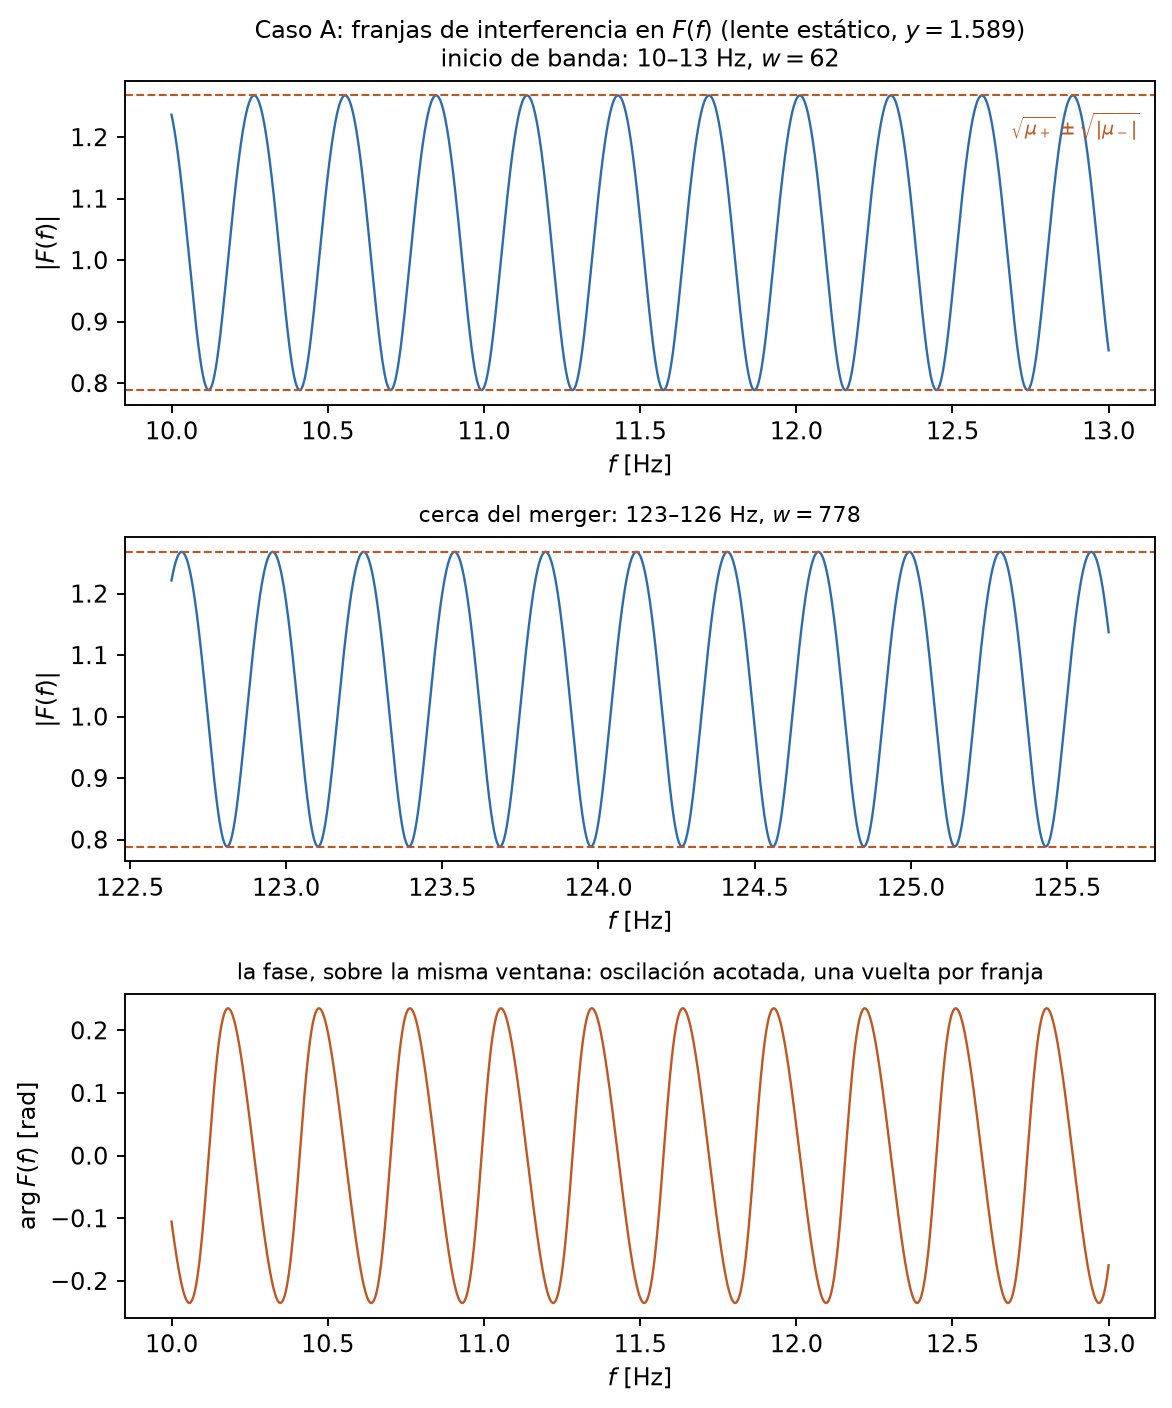
\includegraphics[width=0.85\linewidth]{../cases/case_A_chirp/caseA_F_of_f.png}
\caption{El factor de amplificaci\'on $F(f)$ a trav\'es de toda la banda del
chirp (arriba) y con zoom a 3 Hz (abajo), donde se resuelven las franjas de
interferencia individuales de las dos im\'agenes. $w$ va de 62 (inicio de
banda) a 778 (merger) ac\'a --- muy por encima de donde
\code{tests/test\_waveoptics.py} valida el evaluador r\'apido de \'optica
geom\'etrica contra la forma cerrada exacta a $<4\%$, as\'i que esto es
genuinamente interferencia de ondas, s\'olo demasiado densamente empaquetada
como para resolverse a la escala de banda completa: la transici\'on
chequeada hacia \'optica geom\'etrica a medida que se acerca el merger.}
\end{figure}

\begin{figure}[h]
\centering
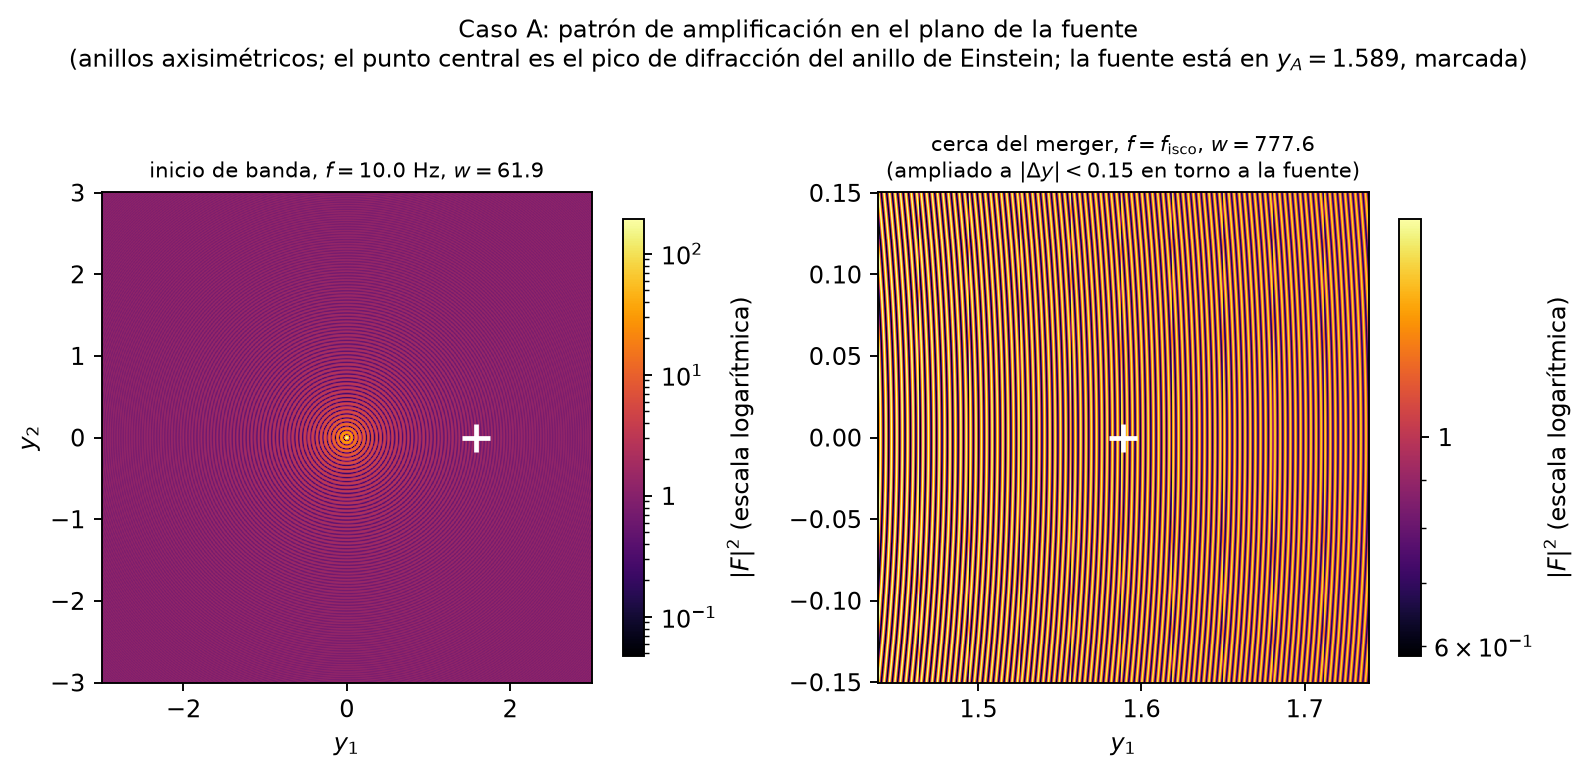
\includegraphics[width=0.85\linewidth]{../cases/case_A_chirp/caseA_diffraction_pattern.png}
\caption{El patr\'on de amplificaci\'on extendido en el plano de la fuente:
anillos de difracci\'on conc\'entricos alrededor del lente con un pico
brillante central de anillo de Einstein (finito en \'optica de ondas, donde
la magnificaci\'on de \'optica geom\'etrica diverge formalmente --- el
an\'alogo en GWs de la mancha \'optica de Arago/Poisson). Izquierda: patr\'on
completo al inicio de banda ($w=61.9$). Derecha: zoom a $|\Delta y|<0.15$
cerca del merger ($w=777.6$) --- los mismos anillos, ahora tan cercanamente
espaciados que parecen franjas casi rectas a este zoom.}
\end{figure}

\begin{figure}[h]
\centering
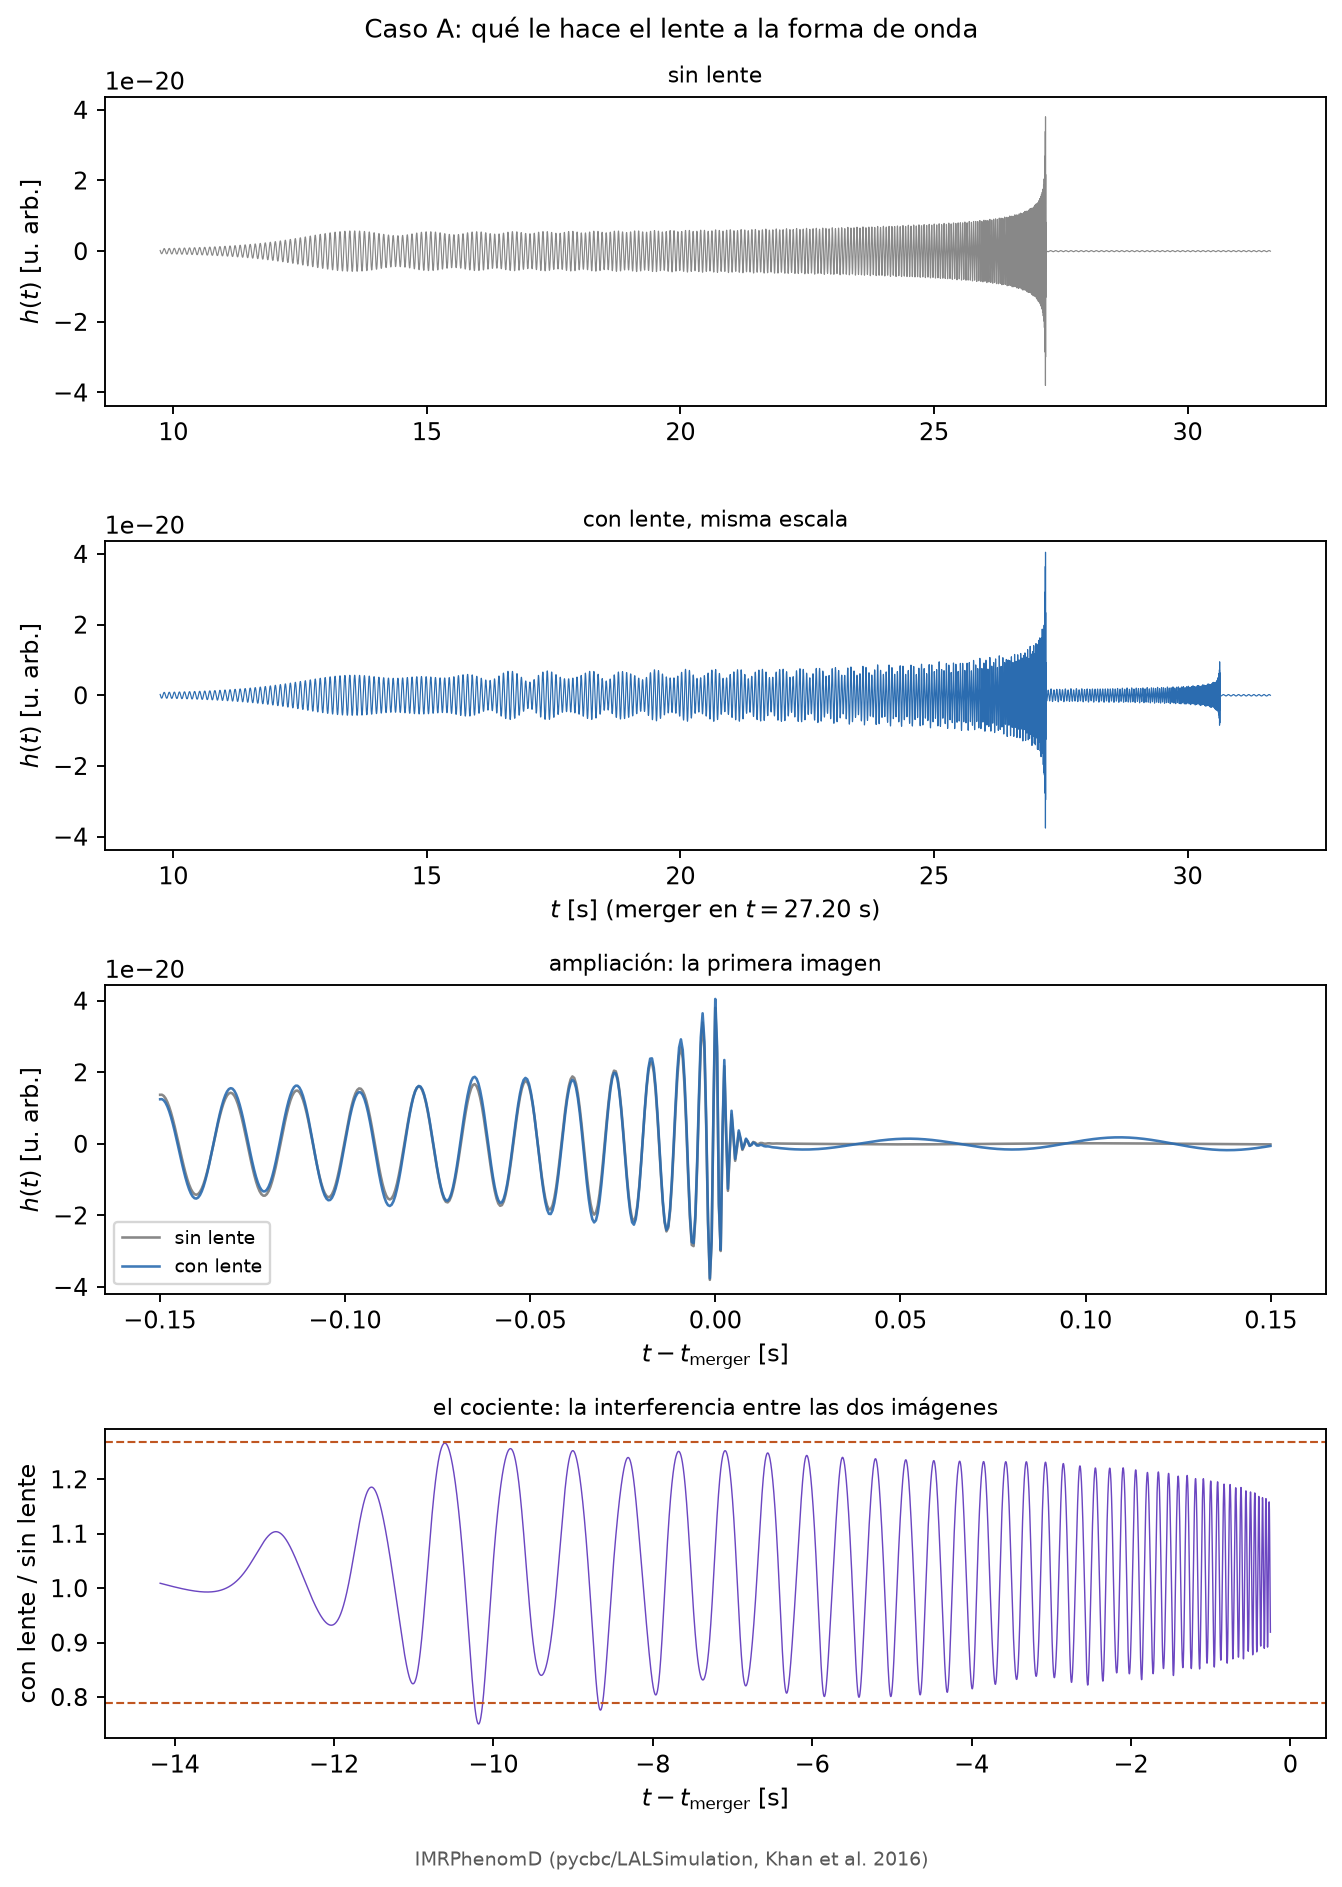
\includegraphics[width=0.9\linewidth]{../cases/case_A_chirp/caseA_strain_time.png}
\caption{Strain lensado vs.\ no lensado en el dominio del tiempo (unidades
arbitrarias, $D_\mathrm{eff}=5$ kpc --- un evento hipot\'etico
ilustrativamente fuerte y cercano, no una distancia realista en tasa de
eventos): vista general extendida m\'as all\'a del merger (arriba), zoom al
merger y ringdown (medio), y zoom al eco de segunda imagen (abajo, ver
texto) --- una r\'eplica m\'as d\'ebil pero reconocible de todo el chirp/
merger/ringdown, exactamente como predice la superposici\'on de im\'agenes
de \'optica geom\'etrica.}
\end{figure}

La amplificaci\'on de la muestra pico es $1.091$ (la muestra $|h(t)|$
individual m\'as grande es mayor lensada que no lensada); la amplificaci\'on
RMS (promediada sobre toda la forma de onda) es $1.056$ --- por el teorema
de Parseval, esta \'ultima depende s\'olo de $|F(f)|$, nunca de la
convenci\'on de fase de Fourier usada.

$F(f)$ modula \textbf{fase} adem\'as de amplitud (figura anterior, subpanel
inferior: $\arg F$ barre un ciclo completo de $2\pi$ aproximadamente una
vez por franja), as\'i que la forma de onda lensada es una copia
\emph{desfasada}, no simplemente reescalada, de la no lensada --- una
afirmaci\'on genuinamente de \'optica de ondas (en el l\'imite de \'optica
geom\'etrica, el lensing \emph{es} s\'olo una magnificaci\'on real).

\paragraph{Una nota sobre causalidad, y un eco genuino.}
El zoom al merger/ringdown de la figura de arriba muestra algo que a
primera vista puede alarmar: el pico lensado combinado se ubica $0.60$~s
\emph{antes} que el no lensado (\code{peak\_time\_lensed\_minus\_unlensed\_s
$=-0.6025$}). Esto \textbf{no} es acausal. La se\~nal lensada del Caso A es
la suma coherente de dos im\'agenes --- una fuerte (tiempo m\'inimo) y una
d\'ebil (punto silla) --- separadas por un retraso \textbf{fijo}
$\Delta T(y_A)=3.434$~s (\code{image\_time\_delay\_seconds}); ambas se
construyen s\'olo a partir del pasado de la fuente. Cerca del merger la
frecuencia barre lo bastante r\'apido como para que la fase de $F(f)$ var\'ie
r\'apidamente a trav\'es de la banda, as\'i que la \emph{interferencia}
entre las dos im\'agenes puede desplazar d\'onde su \emph{suma} alcanza el
pico, sin que llegue informaci\'on antes de tiempo. La confirmaci\'on
independiente, inequ\'ivoca, es el panel inferior de la figura de arriba
(\code{caseA\_detector\_envelope.png}, en \code{cases/case\_A\_chirp/},
muestra la misma confirmaci\'on en escala logar\'itmica sobre toda la
observaci\'on): una segunda copia, genuinamente separada, del
merger/ringdown completo, $\sim$2 \'ordenes de magnitud m\'as d\'ebil,
aparece en
\code{echo\_peak\_time\_s} --- la se\~nal no lensada, en ese mismo
instante, est\'a en su piso de ruido
(\code{echo\_time\_env\_unlensed}$=1.5\times10^{-22}$), mientras la lensada
est\'a $\sim$60 veces por encima (\code{echo\_peak\_env\_lensed}
$=9.65\times10^{-21}$): una se\~nal real, separada, que llega despu\'es,
presente s\'olo por el lente. Predecir ingenuamente su llegada como
$t_\mathrm{peak,no\ lensado}+\Delta T$ falla por $\sim0.6$~s
(\code{echo\_peak\_time\_minus\_prediction\_s$=-0.603$}) --- el
\emph{mismo} desplazamiento de $0.6$~s que el del pico cercano al merger,
a tres cifras: $\Delta T$ aplica desde la llegada de la imagen fuerte
\emph{sola} (libre de interferencia), y el pico combinado usado como su
proxy est\'a desplazado por esa misma interferencia. En vez de asumir una
u otra referencia, \code{run.py} busca directamente el m\'aximo real de la
envolvente lensada y registra tanto el tiempo observado como su diferencia
con la predicci\'on ingenua. Una versi\'on anterior de este an\'alisis
ten\'ia la convenci\'on de signo de Fourier del proyecto invertida, lo que
hac\'ia que esto pareciera genuinamente acausal; v\'ease
\code{wiki/log.md} y \code{wiki/conventions.md}.

\section{Caso B --- cuasi-monocrom\'atico, lente en movimiento}
\label{sec:caseB}

M\'as temprano en el mismo inspiral: $f=0.05$~Hz, con una deriva de s\'olo
$4\%$ sobre una observaci\'on de 24 d\'ias (6 per\'iodos externos), con
60.2 per\'iodos externos todav\'ia por delante antes del merger ---
cuasi-monocrom\'atico. $w_B=0.309$ en todo momento (fijo; s\'olo var\'ia el
par\'ametro de impacto $y(t)$): de lleno en el r\'egimen dominado por
difracci\'on.

\begin{figure}[h]
\centering
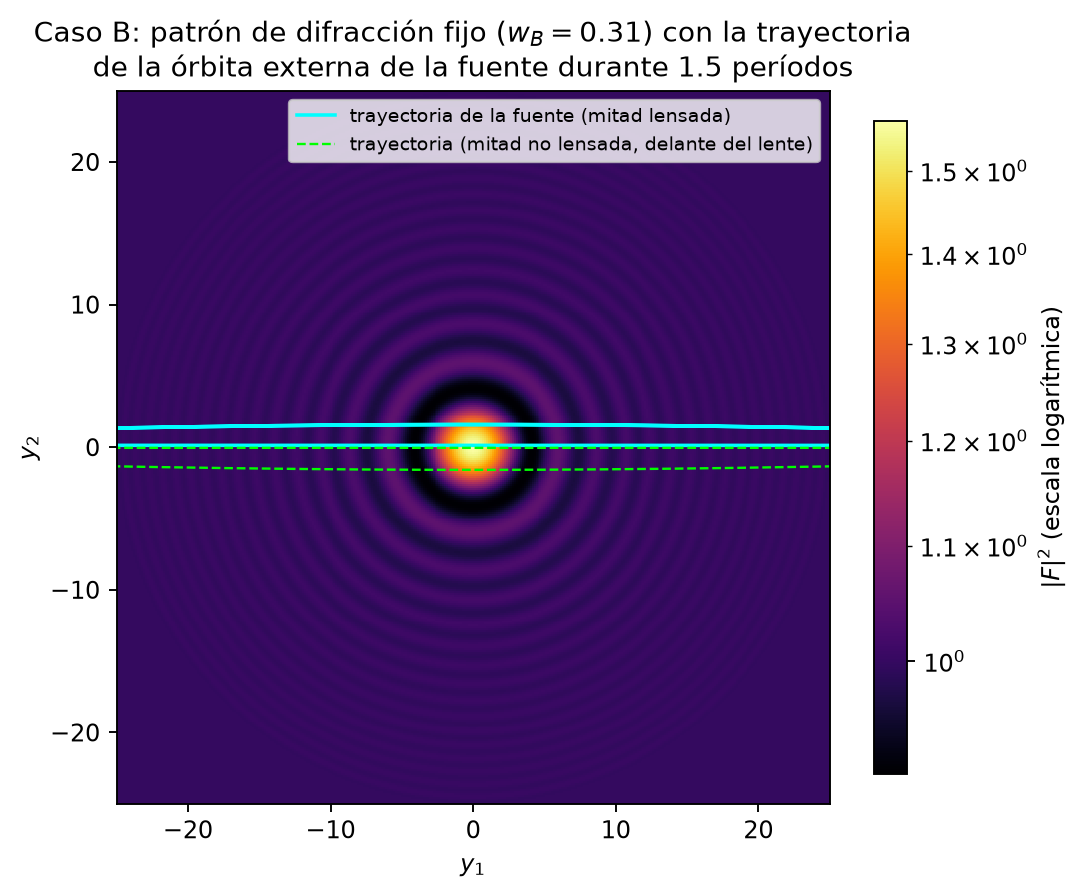
\includegraphics[width=0.85\linewidth]{../cases/case_B_monochromatic/caseB_pattern_with_orbit.png}
\caption{El mismo tipo de patr\'on de difracci\'on fijo que el Caso A (ac\'a
al $w_B=0.309$, mucho m\'as chico) con la traza real de la \'orbita externa
de la fuente, proyectada en el cielo, superpuesta: cian donde la fuente
est\'a lenteada (detr\'as del lente en la l\'inea de visi\'on), verde
punteado donde no lo est\'a (delante de \'el --- v\'ease abajo).}
\end{figure}

\begin{figure}[h]
\centering
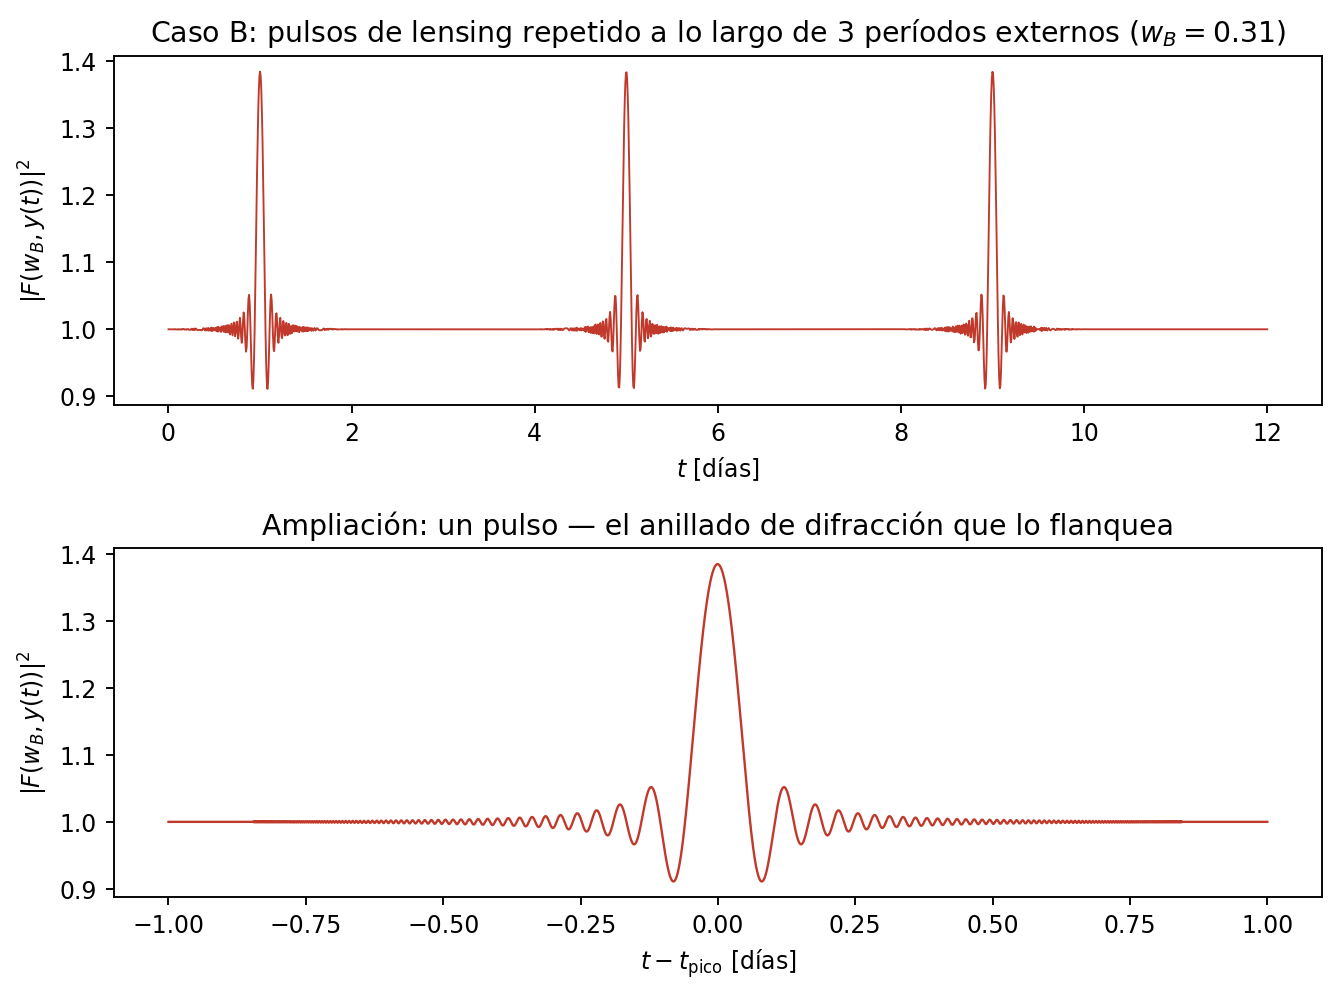
\includegraphics[width=0.85\linewidth]{../cases/case_B_monochromatic/caseB_repeated_pulses.png}
\caption{$|F(w_B,y(t))|^2$ sobre toda la observaci\'on de 24 d\'ias: seis
pulsos de amplificaci\'on peri\'odicos, uno por per\'iodo externo, con pico
en $|F|^2=1.385$, con anillado (`ringing') de difracci\'on visible a ambos
lados de cada pico.}
\end{figure}

Como el lente y la fuente est\'an en el \emph{mismo} sistema en vez de a
las distancias cosmol\'ogicas usuales, bien separadas, $D_{LS}(t)$ la fija
la propia \'orbita externa y se anula dos veces por per\'iodo;
\textbf{exactamente la mitad de la \'orbita resulta no lenteada} (fuente
delante del lente, no detr\'as, as\'i que no existe geometr\'ia de lensing
ah\'i en absoluto --- no es una aproximaci\'on, $F=1$ por construcci\'on).
Este es el origen de los pulsos peri\'odicos de arriba, el an\'alogo en
\'optica de ondas del ``lensing repetido'' encontrado en el l\'imite de
\'optica geom\'etrica por \citet{DOrazioLoeb2020}. Derivaci\'on completa:
\code{theory/theory.pdf} \S4.2--4.3 (que tambi\'en cuantifica exactamente
cu\'anto empuja esto la aproximaci\'on est\'andar de lente delgado, y
muestra que el efecto queda confinado a una ventana de $\sim$60 s por
cruce, coincidente con la regi\'on ya trivial $F\approx1$ --- no una
preocupaci\'on para nada de lo mostrado ac\'a; el Cap.~5 de la teor\'ia
discute qu\'e formalismo har\'ia falta para tratar esa ventana de manera
exacta, y por qu\'e no vale la pena ac\'a).

\begin{figure}[h]
\centering
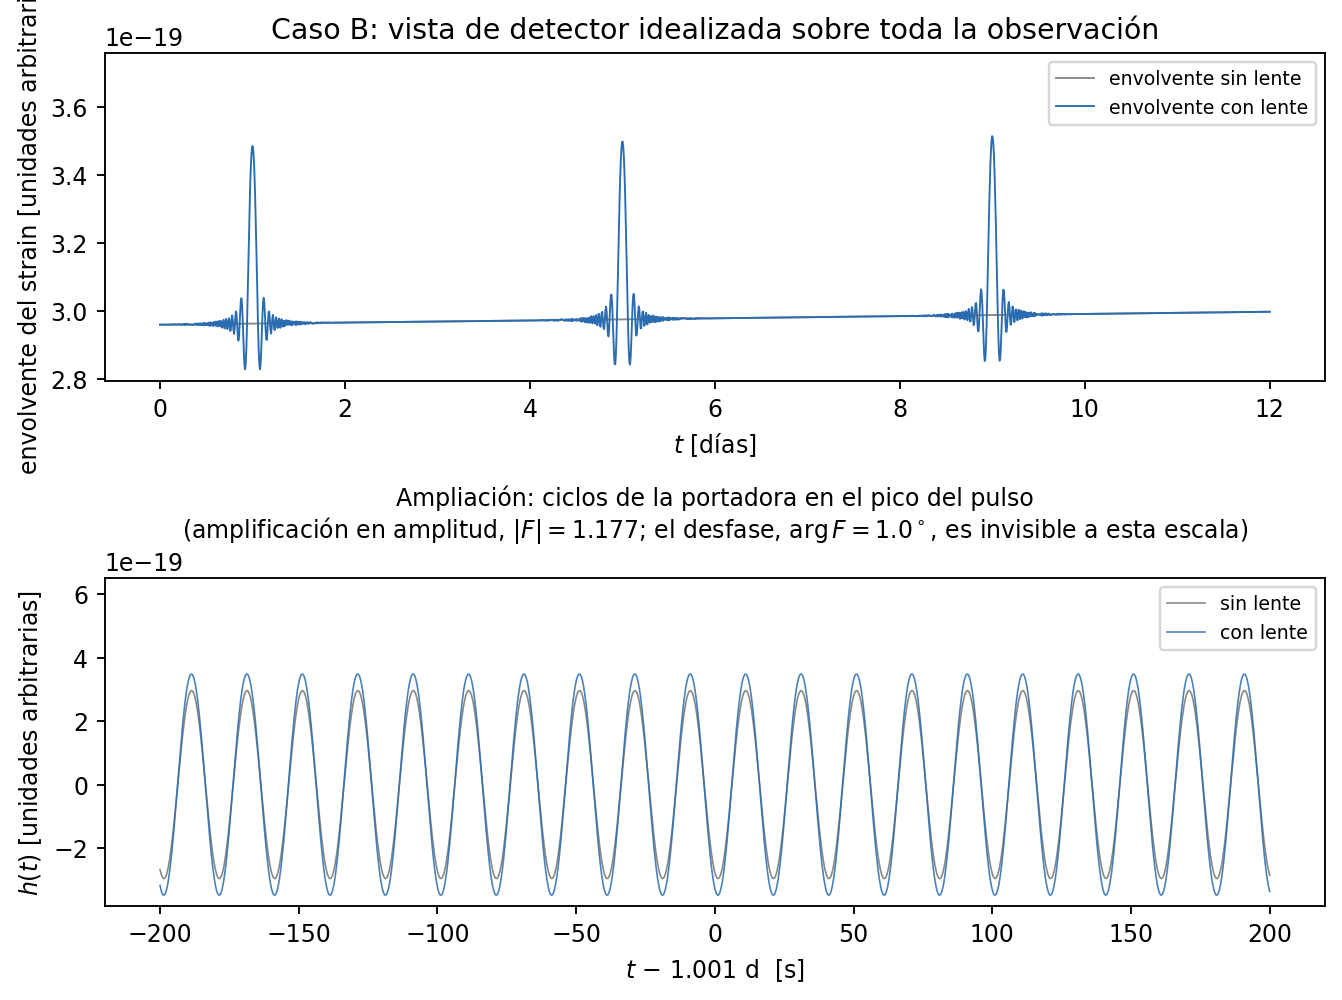
\includegraphics[width=0.9\linewidth]{../cases/case_B_monochromatic/caseB_detector_view.png}
\caption{Vista de detector idealizada. Arriba: envolvente de strain sobre
toda la observaci\'on, seis pulsos limpios montados sobre la portadora que
deriva lentamente. Abajo: una grilla temporal fina con zoom sobre el pico
de un pulso, donde las formas de onda lensada y no lensada se desfasan
visiblemente en un pu\~nado de ciclos de la portadora.}
\end{figure}

\section{Lo que los dos casos muestran juntos}

El mismo lente, el mismo formalismo, dos firmas de aspecto muy distinto,
gobernadas enteramente por una raz\'on de escalas temporales (duraci\'on
del merger vs.\ per\'iodo externo vs.\ duraci\'on de la observaci\'on):

\begin{itemize}
  \item Caso A: un \'unico patr\'on de difracci\'on congelado, muestreado
    en un punto, barrido en \emph{frecuencia} por el propio chirp ---
    franjas de interferencia densas, chequeadas para acercarse al l\'imite
    de \'optica geom\'etrica cuando $w\to\infty$.
  \item Caso B: el mismo tipo de patr\'on, a frecuencia fija, muestreado en
    \emph{tiempo} por el movimiento orbital externo --- pulsos
    peri\'odicos, con exactamente la mitad de la \'orbita no lenteada por
    la propia geometr\'ia del triple.
  \item Ambos casos: el lensing no es simplemente ``hacerlo m\'as
    brillante''. $F(f)$ (o $F(t)$) es complejo, y su fase deja una marca
    real, verificable, en la forma de onda m\'as all\'a de una amplitud
    global.
\end{itemize}

\section{Alcance y limitaciones}

Declaradas expl\'icitamente, no dejadas impl\'icitas (cada una tambi\'en
registrada en \code{wiki/log.md} en el momento en que se decidi\'o):
\begin{itemize}
  \item S\'olo lente de masa puntual; sin distribuci\'on de masa extendida.
  \item IMRPhenomD (Caso A) es un modelo calibrado, no re-derivado ac\'a; el
    generador de respaldo TaylorF2 est\'a truncado en 2PN y no tiene
    merger/ringdown; la evoluci\'on de frecuencia subyacente del Caso B es
    s\'olo de orden dominante.
  \item Sin calibraci\'on absoluta de strain (los prefactores de
    inclinaci\'on/polarizaci\'on quedan plegados en una constante de orden
    $1$) --- s\'olo las amplitudes relativas y el factor de amplificaci\'on
    de lensing son afirmaciones f\'isicas ac\'a.
  \item La vista de detector idealizada no tiene ruido, patr\'on de antena,
    ni filtrado adaptado --- s\'olo ilustrativa, seg\'un el alcance
    definido desde el principio.
  \item La aproximaci\'on de lente delgado/paraxial se empuja de manera
    cuantificable cerca de cada cruce de frente/atr\'as del Caso B
    (\S\ref{sec:caseB}); se muestra que no afecta nada de lo reportado.
\end{itemize}

\bibliographystyle{plainnat}
\bibliography{../theory/refs}

\end{document}
